% Preamble templated from Dhawal24112006/EE1030
\documentclass{beamer}
\mode<presentation>
\usepackage{amsmath}
\usepackage{amssymb}
% \usepackage{advdate}
\usepackage{adjustbox}
\usepackage{subcaption}
% \usepackage{enumitem}
\usepackage{multicol}
\usepackage{mathtools}
\usepackage{tikz}
\usetikzlibrary{positioning, arrows.meta}
\usepackage{listings}
\usepackage{xcolor}
\usepackage{url}
% \def\UrlBreaks{\do\/\do-}
\usetheme{Boadilla}
\usecolortheme{lily}
\setbeamertemplate{footline}
{
  \leavevmode%
  \hbox{%
  \begin{beamercolorbox}[wd=\paperwidth,ht=2.25ex,dp=1ex,right]{author in head/foot}%
    \insertframenumber{} / \inserttotalframenumber\hspace*{2ex}
  \end{beamercolorbox}}%
  \vskip0pt%
}
\setbeamertemplate{navigation symbols}{}

\providecommand{\nCr}[2]{\,^{#1}C_{#2}} % nCr
\providecommand{\nPr}[2]{\,^{#1}P_{#2}} % nPr
\providecommand{\mbf}{\mathbf}
\providecommand{\pr}[1]{\ensuremath{\Pr\left(#1\right)}}
\providecommand{\qfunc}[1]{\ensuremath{Q\left(#1\right)}}
\providecommand{\sbrak}[1]{\ensuremath{{}\left[#1\right]}}
\providecommand{\lsbrak}[1]{\ensuremath{{}\left[#1\right.}}
\providecommand{\rsbrak}[1]{\ensuremath{{}\left.#1\right]}}
\providecommand{\brak}[1]{\ensuremath{\left(#1\right)}}
\providecommand{\lbrak}[1]{\ensuremath{\left(#1\right.}}
\providecommand{\rbrak}[1]{\ensuremath{\left.#1\right)}}
\providecommand{\cbrak}[1]{\ensuremath{\left\{#1\right\}}}
\providecommand{\lcbrak}[1]{\ensuremath{\left\{#1\right.}}
\providecommand{\rcbrak}[1]{\ensuremath{\left.#1\right\}}}
\theoremstyle{remark}
\newtheorem{rem}{Remark}
\newcommand{\sgn}{\mathop{\mathrm{sgn}}}
\providecommand{\abs}[1]{\left\vert#1\right\vert}
\providecommand{\res}[1]{\Res\displaylimits_{#1}}
\providecommand{\norm}[1]{\lVert#1\rVert}
\providecommand{\mtx}[1]{\mathbf{#1}}
\providecommand{\mean}[1]{E\left[ #1 \right]}
\providecommand{\fourier}{\overset{\mathcal{F}}{ \rightleftharpoons}}
\providecommand{\system}{\overset{\mathcal{H}}{ \longleftrightarrow}}
\providecommand{\dec}[2]{\ensuremath{\overset{#1}{\underset{#2}{\gtrless}}}}
\newcommand{\myvec}[1]{\ensuremath{\begin{pmatrix}#1\end{pmatrix}}}
\let\vec\mathbf

\definecolor{commentgreen}{RGB}{2,112,10}
\definecolor{eminence}{RGB}{108,48,130}
\definecolor{weborange}{RGB}{255,165,0}
\definecolor{frenchplum}{RGB}{129,20,83}
\definecolor{backcolour}{RGB}{248,248,248}
\definecolor{codegray}{RGB}{128,128,128}

% Configure the Python style
\lstdefinestyle{pythonstyle}{
    language=Python,
    backgroundcolor=\color{backcolour},   
    commentstyle=\color{commentgreen}\itshape,
    keywordstyle=\color{eminence}\bfseries,
    numberstyle=\tiny\color{codegray},
    stringstyle=\color{weborange},
    basicstyle=\ttfamily\footnotesize,
    breakatwhitespace=false,         
    breaklines=true,                 % Wraps long lines
    captionpos=b,                    % Sets the caption-position to bottom
    keepspaces=true,                 % Preserves spaces in text
    numbers=left,                    % Line numbers on the left
    numbersep=5pt,                   
    showspaces=false,                
    showstringspaces=false,          % Removes weird underscores in strings
    showtabs=false,                  
    tabsize=4,
    frame=single,                    % Adds a border around the code
    rulecolor=\color{lightgray},     % Border color
    % Extra Python specific styling
    emph={self, cls, @classmethod, @staticmethod, @property}, 
    emphstyle=\color{frenchplum}\bfseries
}

\lstset{
frame=single,
breaklines=true,
columns=fullflexible,
showstringspaces=false,
style=pythonstyle
}

\numberwithin{equation}{section}

\title{POMPS Presentation: 1.2.83}
\author{Subhodeep Chakraborty \\ ee25btech11055,\\IIT Hyderabad.}
\date{\today}

\begin{document}

\begin{frame}
    \titlepage
\end{frame}
\begin{frame}
    \tableofcontents
\end{frame}


\section{Problem Statement}
\begin{frame}{Problem Statement}
    \textbf{Question 1.2.83 (CS 2008)} \\
        The Newton-Raphson iteration $x_{n+1} = \frac{1}{2}\left(x_n + \frac{R}{x_n}\right)$ can be used to compute the
        \begin{enumerate}[a)]
            \item square of $R$
            \item reciprocal of $R$
            \item square root of $R$
            \item logarithm of $R$
        \end{enumerate}
    %\end{block}
\end{frame}

\section{Limit Analysis}
\begin{frame}{Method 1: Steady-State / Limit Analysis}
    If the sequence $x_n$ converges to a limit $L$ as $n \to \infty$, then we can state that the steady-state holds:
    \begin{align}
        \lim_{n \to \infty} x_{n+1} &= \lim_{n \to \infty} x_n = L
    \end{align}
    Substituting this into the given iteration equation:
    \begin{align}
        L &= \frac{1}{2}\left(L + \frac{R}{L}\right) \\
        2L &= L + \frac{R}{L} \\
        L &= \frac{R}{L} \\
        L^2 &= R \implies L = \sqrt{R}
    \end{align}
    Thus, the iteration computes the square root of $R$. \\
    \textbf{Answer: (c)}
\end{frame}
\section{Reverse Newton-Raphson}
\begin{frame}{Method 2: Reverse-Engineering Newton-Raphson}
    The generalized Newton-Raphson formula for finding roots of $f(x) = 0$ is:
    \begin{align}
        x_{n+1} &= x_n - \frac{f(x_n)}{f'(x_n)}
    \end{align}
    On manipulating the given expression into this standard form:
    \begin{align}
        x_{n+1} &= \frac{x_n}{2} + \frac{R}{2x_n} \\
        x_{n+1} &= x_n - x_n + \frac{x_n}{2} + \frac{R}{2x_n} \\
        x_{n+1} &= x_n - \left( \frac{x_n}{2} - \frac{R}{2x_n} \right) \\
        x_{n+1} &= x_n - \frac{x_n^2 - R}{2x_n}
    \end{align}
\end{frame}

\begin{frame}{Method 2: Reverse-Engineering Newton-Raphson}
    Comparing with the standard N-R formula:
    \begin{align}
        \frac{f(x_n)}{f'(x_n)} &= \frac{x_n^2 - R}{2x_n}
    \end{align}
    By observation, if we set the numerator to be the function and the denominator to be its derivative:
    \begin{align}
        f(x) &= x^2 - R \\
        f'(x) &= 2x 
    \end{align}
    The Newton-Raphson method finds the roots of $f(x) = 0$. 
    \begin{align}
        x^2 - R &= 0 \implies x = \sqrt{R}
    \end{align}
    This confirms it evaluates the square root of R.
\end{frame}
\section{Fixed-Point Theorem}
\begin{frame}{Method 3: Fixed-Point Theorem \& Cobweb Plot}
    The given sequence $x_{n+1} = \frac{1}{2}\left(x_n + \frac{R}{x_n}\right)$ can be written as a fixed-point iteration function:
    \begin{align}
        x_{n+1} &= g(x_n)
    \end{align}
    where $g(x) = \frac{1}{2}\left(x + \frac{R}{x}\right)$.
    
    \vspace{0.5cm}
    For a fixed-point iteration to converge to a limit $L$, two things must be true:
    \begin{itemize}
        \item \textbf{The Fixed Point:} The limit must satisfy $L = g(L)$. Graphically, this is where the curve $y = g(x)$ intersects the identity line $y = x$.
    \end{itemize}
\end{frame}

\begin{frame}{Method 3: Fixed-Point Theorem \& Cobweb Plot}
    \begin{itemize}
        \item \textbf{The Convergence Condition (Stability):} The derivative of $g(x)$ at the root must have an absolute value less than 1, meaning $\abs{g'(L)} < 1$.
    \end{itemize}
    
    Let's find the derivative of $g(x)$:
    \begin{align}
        g'(x) &= \frac{1}{2}\left(1 - \frac{R}{x^2}\right)
    \end{align}
    
    At the root $x = \sqrt{R}$, the derivative is:
    \begin{align}
        g'\left(\sqrt{R}\right) &= \frac{1}{2}\left(1 - \frac{R}{(\sqrt{R})^2}\right) = 0
    \end{align}
    
    Because the derivative is exactly zero, this rigorously proves not just convergence, but \textbf{quadratic (superlinear) convergence}.
\end{frame}
\begin{frame}{Proof of Quadratic Convergence}
    With the derived condition $g'(L) = 0$, we analyse the error $e_n = x_n - L$. 
    
    \vspace{0.3cm}
    The error at the next step is:
    \begin{align}
        e_{n+1} &= x_{n+1} - L = g(x_n) - L \\
        e_{n+1} &= g(L + e_n) - L
    \end{align}
    
    Expanding $g(L + e_n)$ using a Taylor series around the root $L$:
    \begin{align}
        g(L + e_n) &= g(L) + g'(L)e_n + \frac{g''(c)}{2!}e_n^2
    \end{align}
    where $c$ is a value between $L$ and $x_n$.
\end{frame}

\begin{frame}{Proof of Quadratic Convergence}
    We apply our known conditions at the fixed point: $g(L) = L$ and the derivative condition $g'(L) = 0$.
    
    \vspace{0.3cm}
    Substituting these into the Taylor expansion:
    \begin{align}
        g(L + e_n) &= L + (0)e_n + \frac{g''(c)}{2}e_n^2 \\
        g(L + e_n) &= L + \frac{g''(c)}{2}e_n^2
    \end{align}
    
    Substituting back into our error equation $e_{n+1} = g(L + e_n) - L$:
    \begin{align}
        e_{n+1} &= \frac{g''(c)}{2}e_n^2 \implies \abs{e_{n+1}} = \abs{\frac{g''(c)}{2}} \abs{e_n}^2
    \end{align}
    
    Since $\abs{e_{n+1}} \propto \abs{e_n}^2$, the error is squared at each step, proving \textbf{quadratic convergence}.
\end{frame}
\iffalse
\begin{frame}{Method 3: Dynamical Systems / State-Space Approach}
    We can model this as a coupled discrete-time dynamical system. Let us introduce a secondary state variable $y_n = \frac{R}{x_n}$. \\
    The system maps $\vec{v}_n \to \vec{v}_{n+1}$ where $\vec{v}_n = \myvec{x_n \\ y_n}$.
    
    The update for $x_n$ is the Arithmetic Mean (AM):
    \begin{align}
        x_{n+1} &= \frac{1}{2}(x_n + y_n)
    \end{align}
    The corresponding update for $y_n$ is the Harmonic Mean (HM):
    \begin{align}
        y_{n+1} &= \frac{R}{x_{n+1}} = \frac{2R}{x_n + y_n} = \frac{2 x_n y_n}{x_n + y_n}
    \end{align}
\end{frame}

\begin{frame}{Method 3: Dynamical Systems / State-Space Approach}
    This forms the classic \textbf{Arithmetic-Harmonic Mean (AHM)} iteration. 
    Notice the invariant property of the state vector:
    \begin{align}
        x_n y_n = R \quad \forall n
    \end{align}
    As $n \to \infty$, the AM and HM bounds squeeze together, forcing the system to an equilibrium state where $x_\infty = y_\infty$.
    
    Substituting the equilibrium condition into our invariant:
    \begin{align}
        x_\infty y_\infty &= R \\
        x_\infty^2 &= R \\
        x_\infty &= \sqrt{R}
    \end{align}
    Both state variables independently converge to the Geometric Mean of the initial states, which is $\sqrt{R}$.
\end{frame}

\begin{frame}{Convergence Error Analysis (Rigorous Proof)}
    To rigorously prove global convergence from a signal processing perspective, define a normalized error signal $e_n$:
    \begin{align}
        e_n &= \frac{x_n - \sqrt{R}}{x_n + \sqrt{R}}
    \end{align}
    Applying the system transformation to $e_{n+1}$:
    \begin{align}
        e_{n+1} &= \frac{x_{n+1} - \sqrt{R}}{x_{n+1} + \sqrt{R}} = \frac{\frac{1}{2}\left(x_n + \frac{R}{x_n}\right) - \sqrt{R}}{\frac{1}{2}\left(x_n + \frac{R}{x_n}\right) + \sqrt{R}} \\
        e_{n+1} &= \frac{x_n^2 + R - 2x_n\sqrt{R}}{x_n^2 + R + 2x_n\sqrt{R}} = \left(\frac{x_n - \sqrt{R}}{x_n + \sqrt{R}}\right)^2 \\
        e_{n+1} &= e_n^2
    \end{align}
    Since $e_n \to e_0^{2^n}$, for any initial guess $x_0 > 0$, $\abs{e_0} < 1 \implies e_\infty = 0$, confirming absolute quadratic convergence to $\sqrt{R}$.
\end{frame}
\fi

\section{Python Codes}
\begin{frame}[fragile,allowframebreaks]{Python Implementation}
    \lstinputlisting[basicstyle=\scriptsize\ttfamily]{../codes/plot.py}
\end{frame}

\section{Simulation Verification}
% Method 1: Convergence Plot
\begin{frame}{Method 1: Sequence Convergence}
    This plot shows the iteration sequence $x_{n+1} = \frac{1}{2}\left(x_n + \frac{25}{x_n}\right)$ for three different initial guesses. 
    
    While the standard ($x_0 = 12$) and small ($x_0 = 0.5$) guesses converge to the positive root $\sqrt{25} = 5.0$, the negative guess ($x_0 = -12$) correctly converges to the alternate valid root $-5.0$.
    \begin{center}
        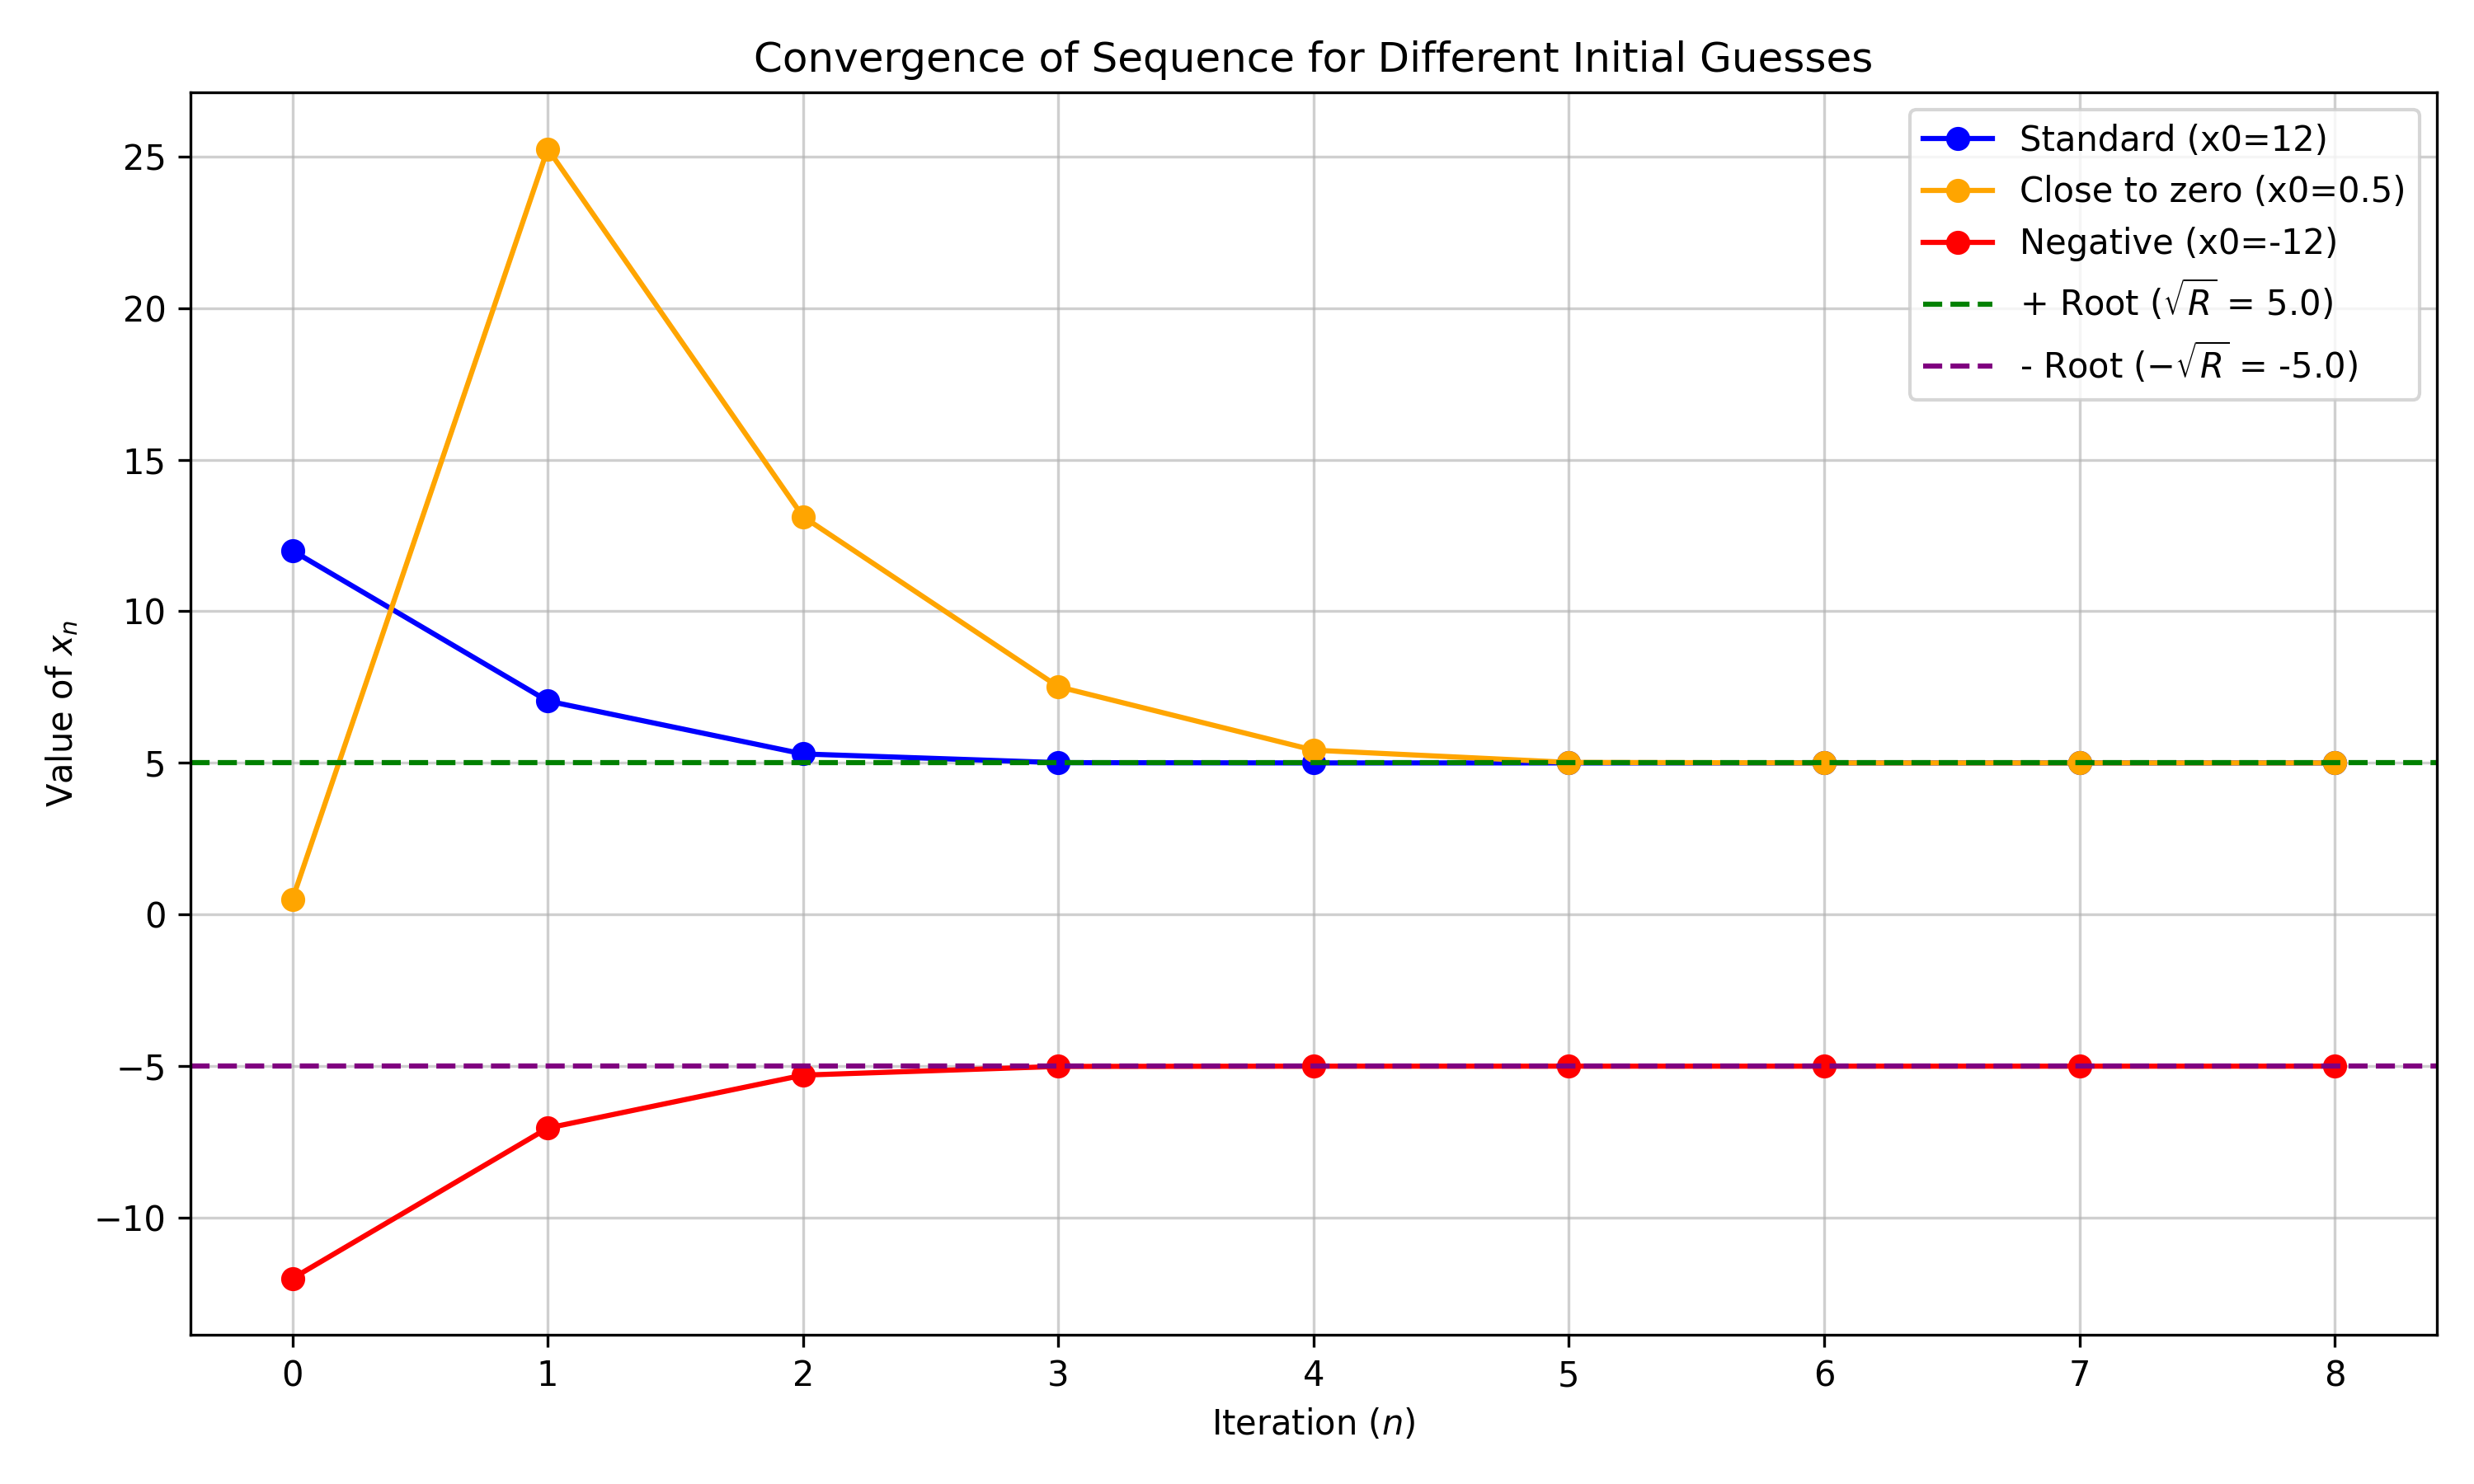
\includegraphics[width=0.8\textwidth]{../figs/plot1_convergence_multi.png}
    \end{center}
\end{frame}

% Method 1: Error Plot
\begin{frame}{Method 1: Absolute Error Analysis}
    This semi-log plot visualizes the absolute error over iterations. Despite differing initial trajectories (especially the initial spike for the $x_0 = 0.5$ guess), all paths eventually lock into a steep, parabolic downward curve. 
    
    This uniform drop-off is the hallmark of \textbf{super-linear (quadratic) convergence}.
    \begin{center}
        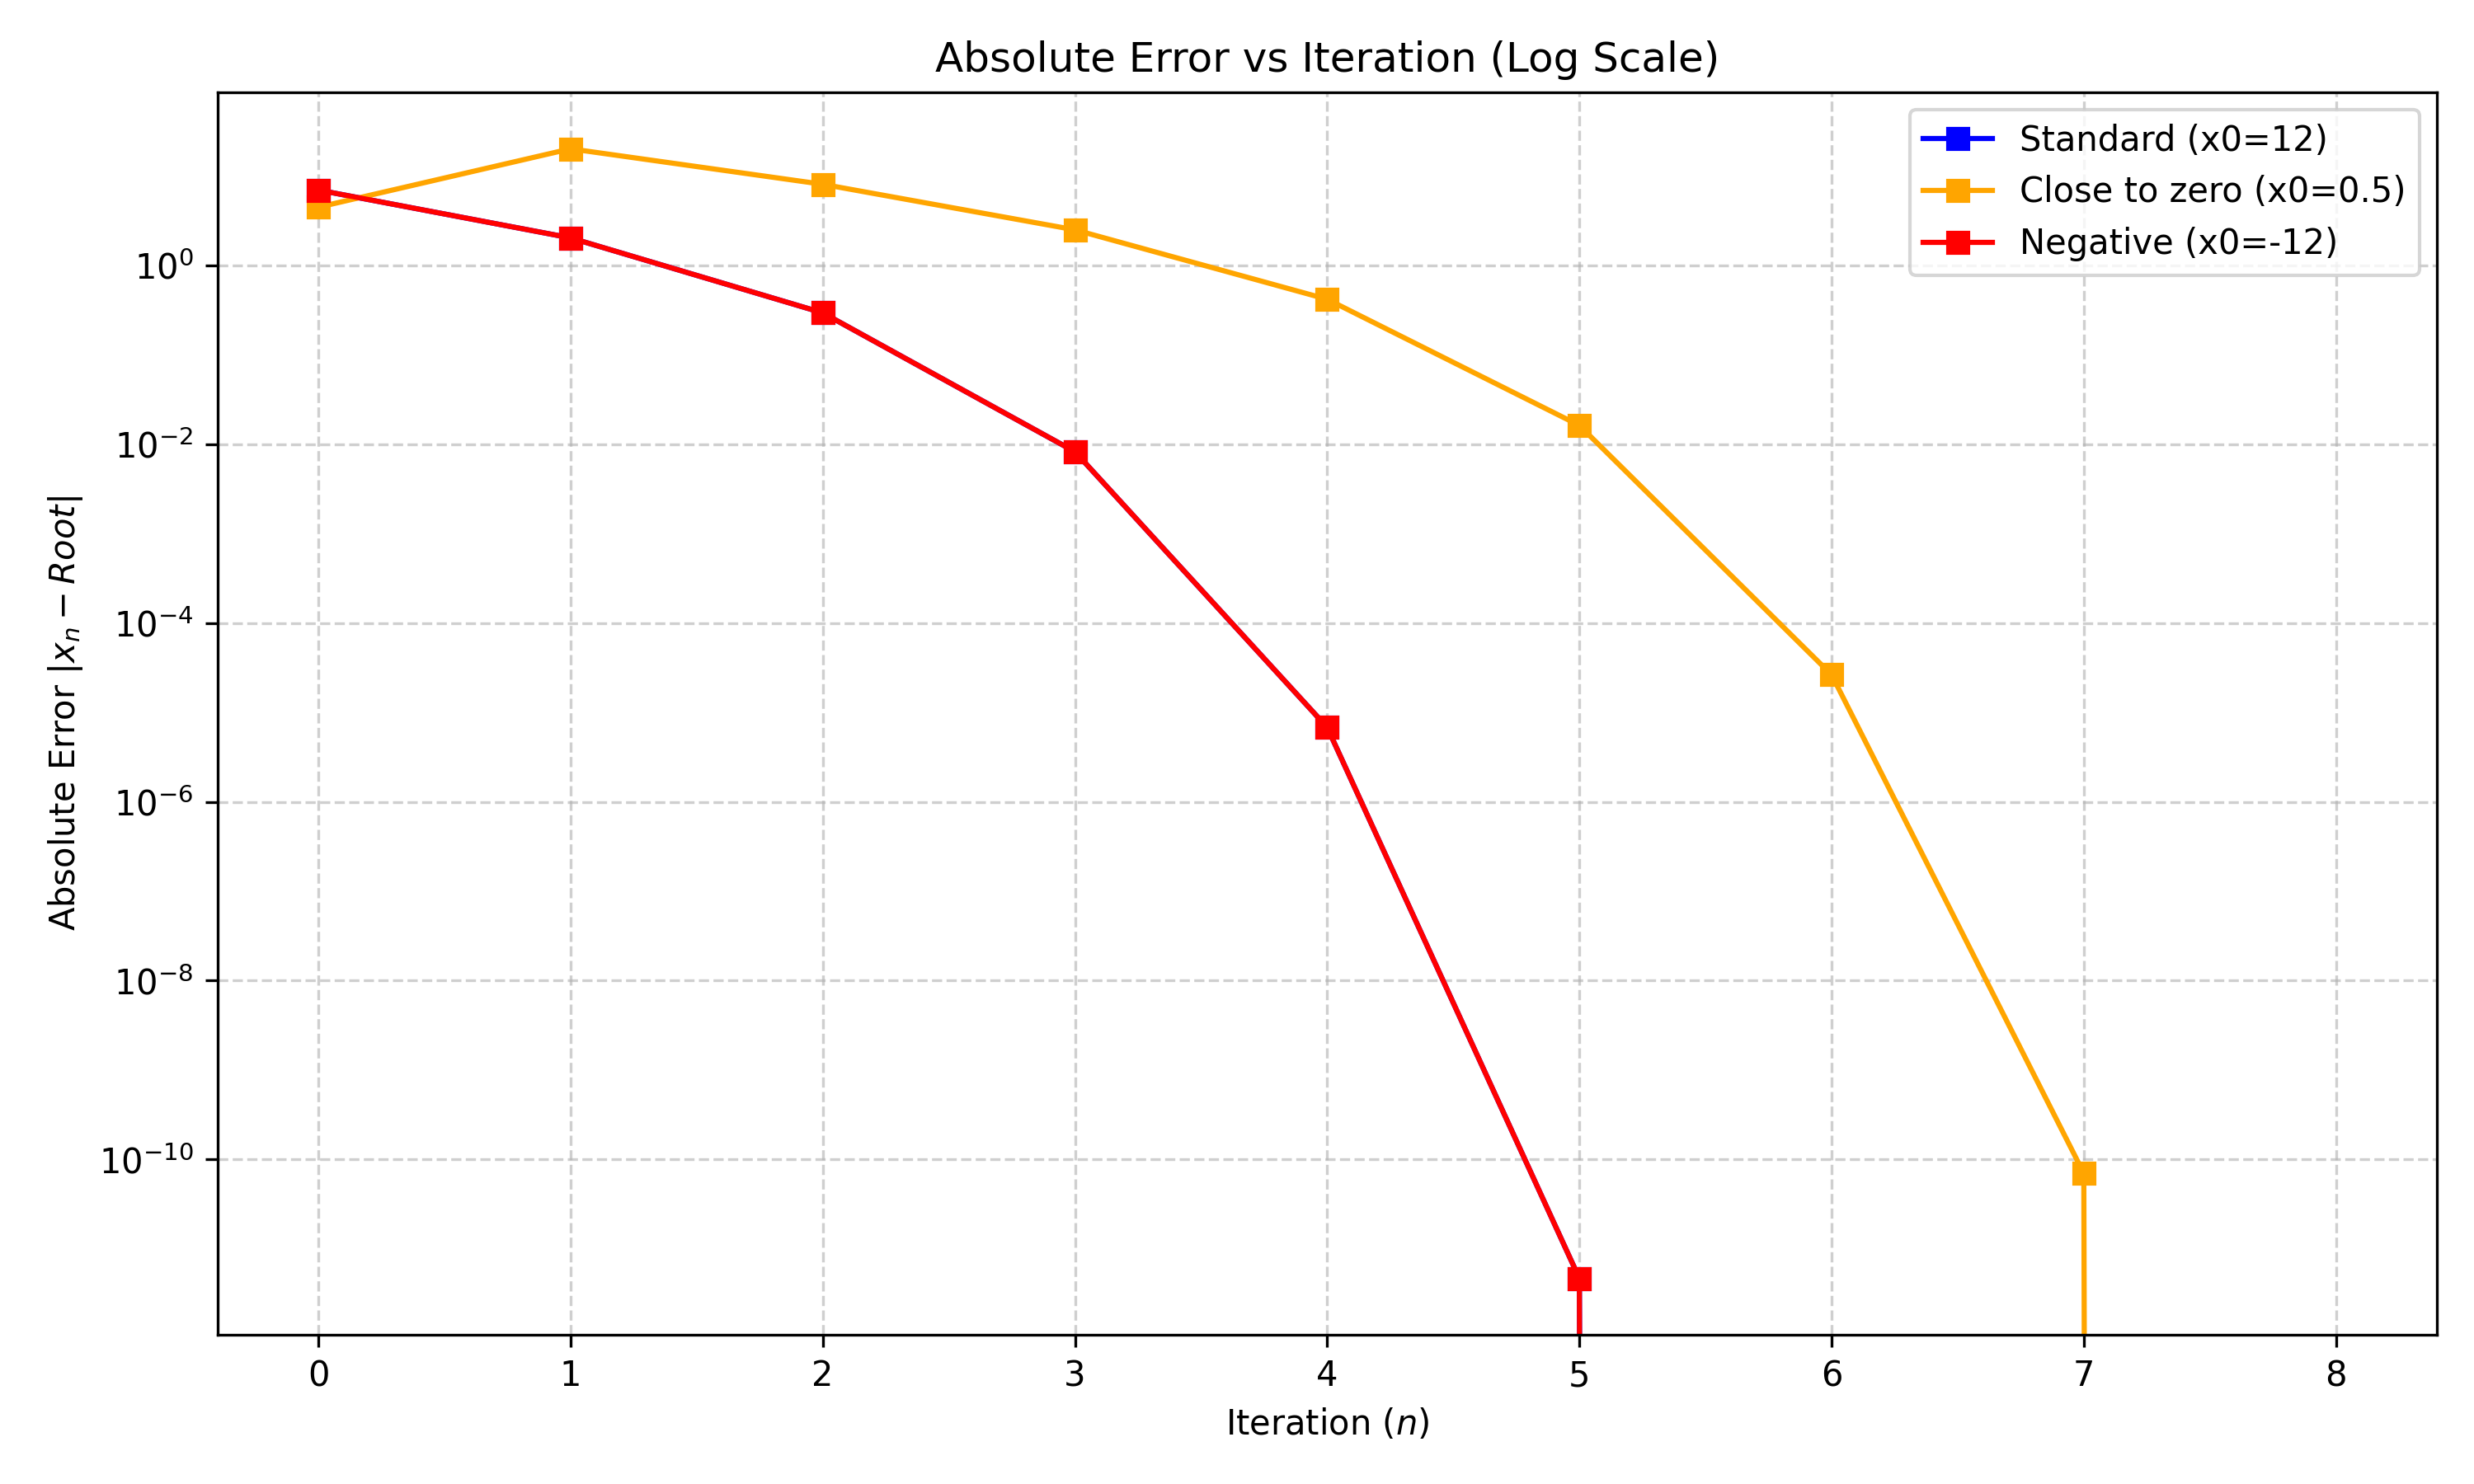
\includegraphics[width=0.8\textwidth]{../figs/plot2_error_multi.png}
    \end{center}
\end{frame}

% Method 2: Geometric Execution
\begin{frame}{Method 2: Geometric Execution}
    This figure visualizes the geometric root-finding process on the function $f(x) = x^2 - R$ for a standard initial guess ($x_0 = 12$). 
    
    The tangent line physically illustrates the Newton-Raphson relationship $x_{n+1} = x_n - \frac{f(x_n)}{f'(x_n)}$, showing the aggressive mathematical jump toward the true root.
    \begin{center}
        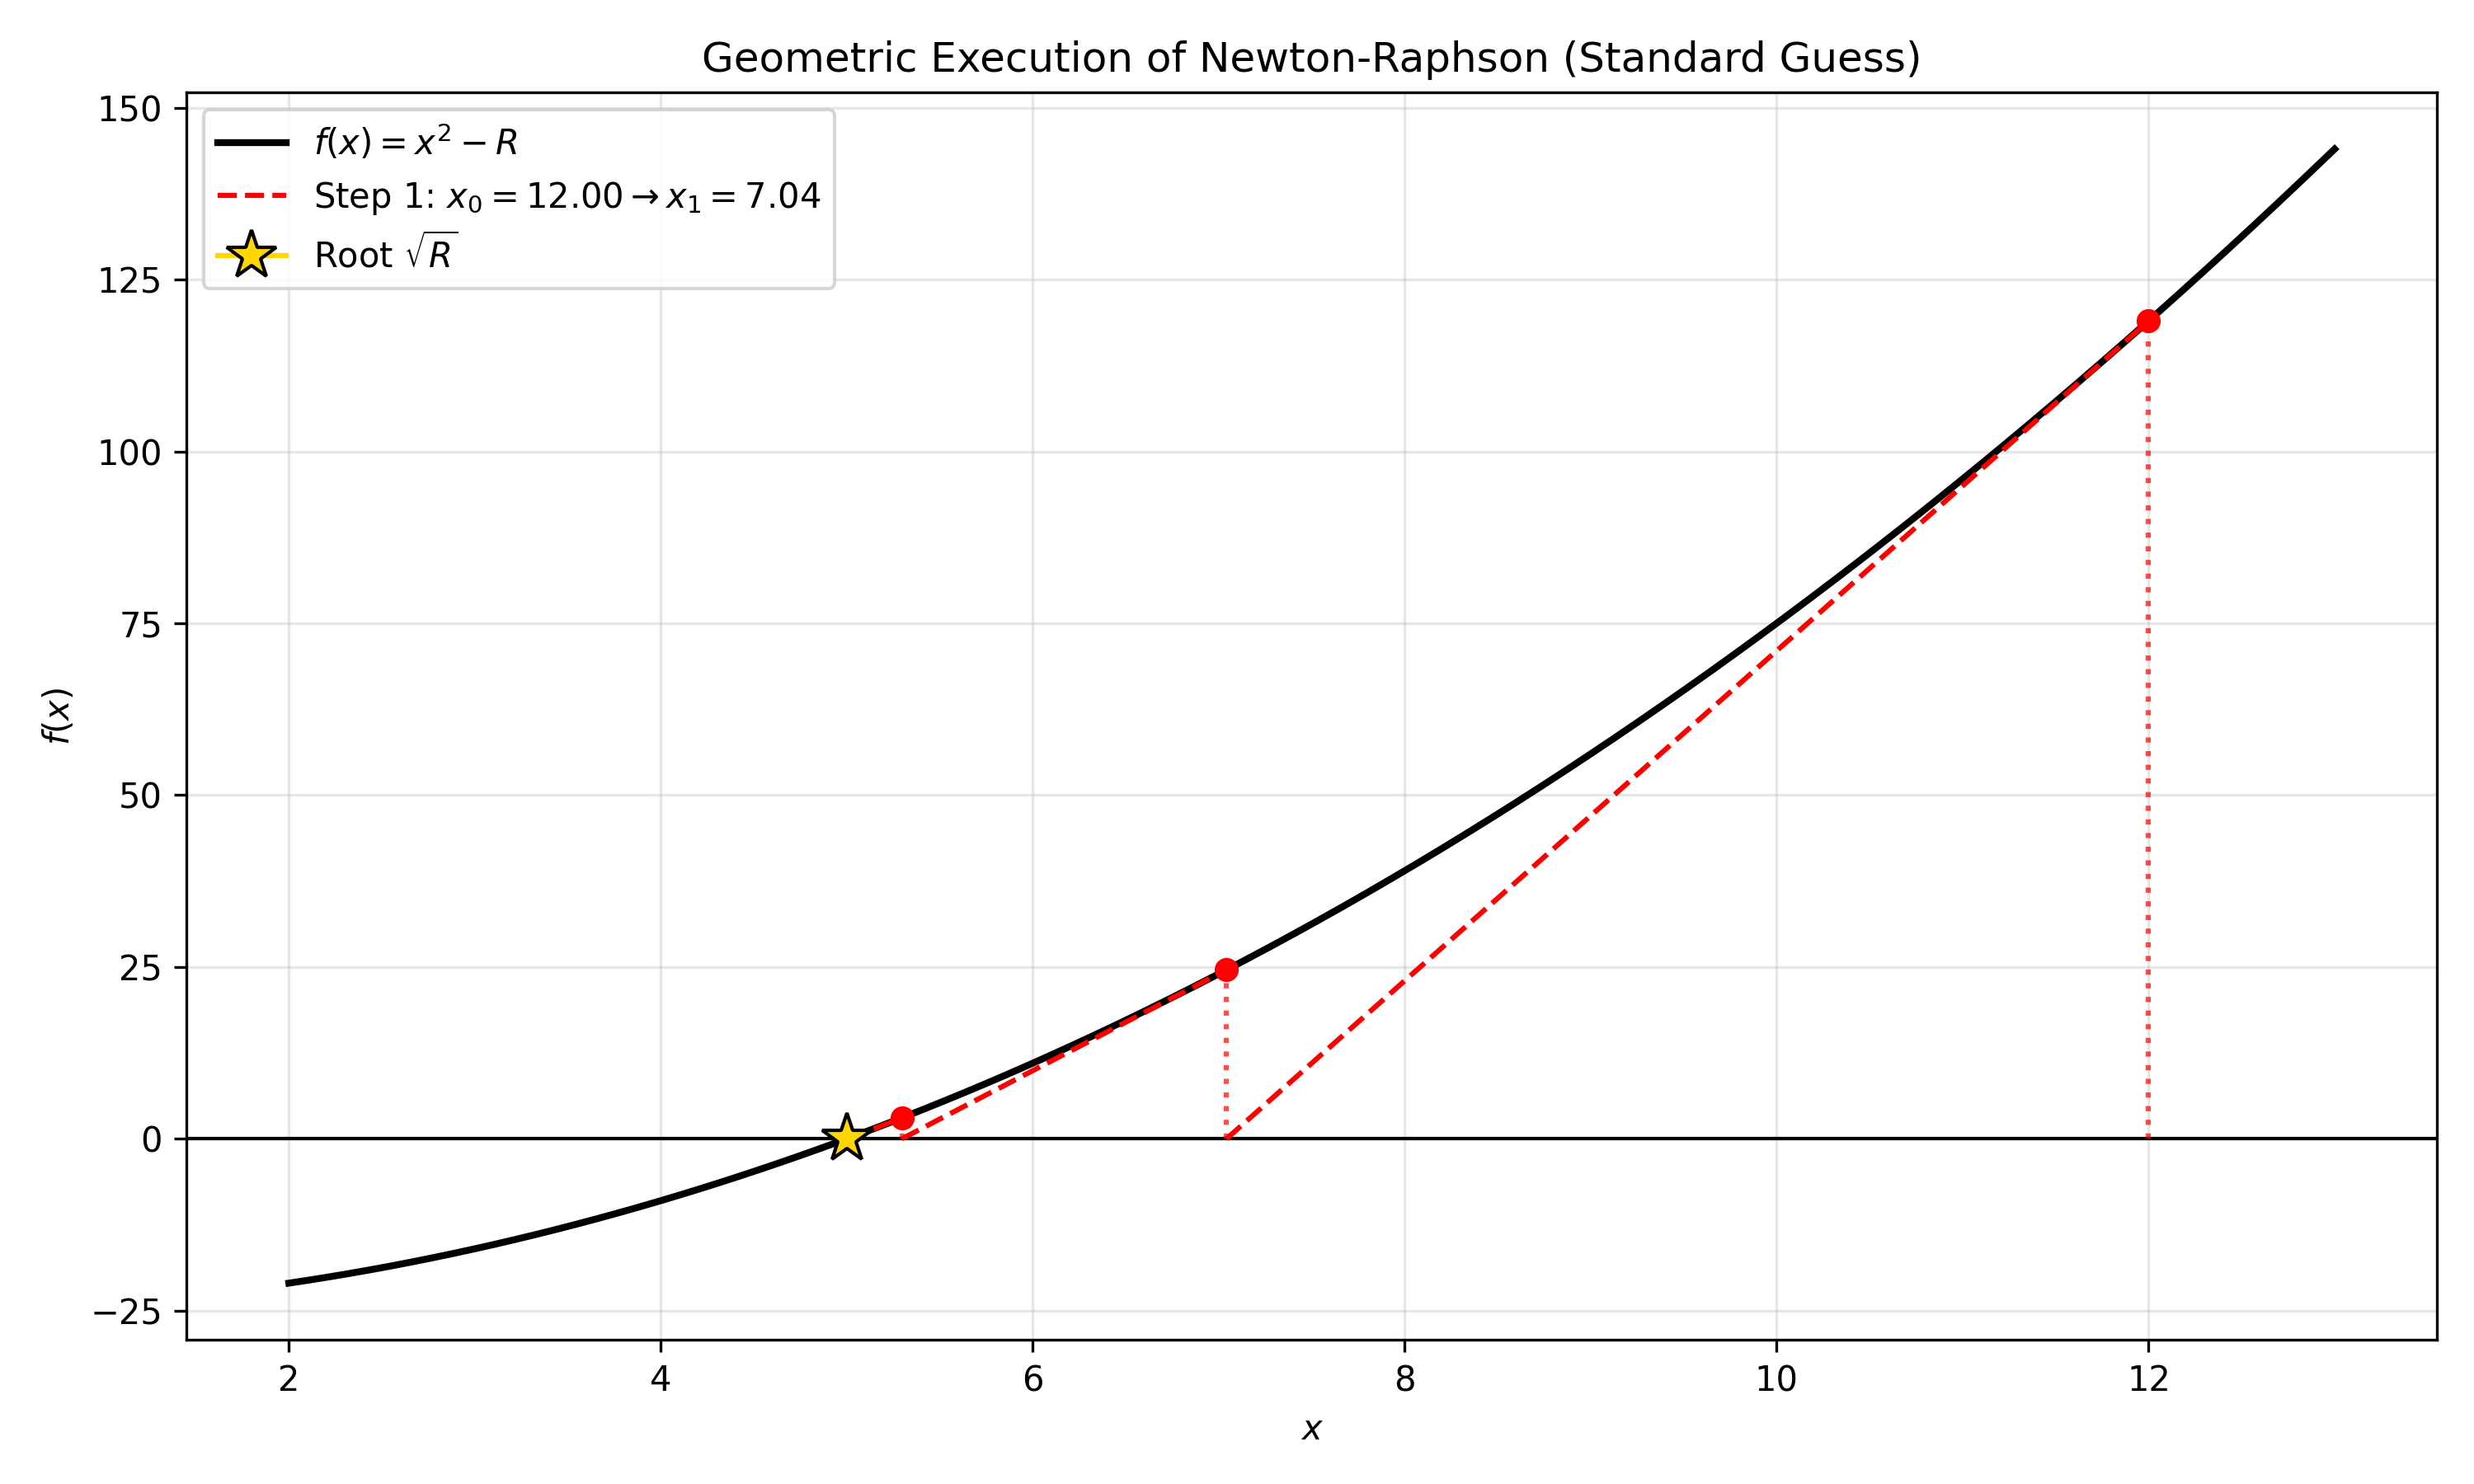
\includegraphics[width=0.8\textwidth]{../figs/plot3_geometric_nr.png}
    \end{center}
\end{frame}
% Method 3: Cobweb Plot (Standard)
\begin{frame}{Method 3: Cobweb Plot (Standard Guess)}
    This cobweb diagram traces the fixed-point iteration for $x_0 = 12$. The sequence updates by bouncing between the curve $y = g(x)$ and the identity line $y = x$, visually funneling directly into the fixed point at $x = 5$.
    \begin{center}
        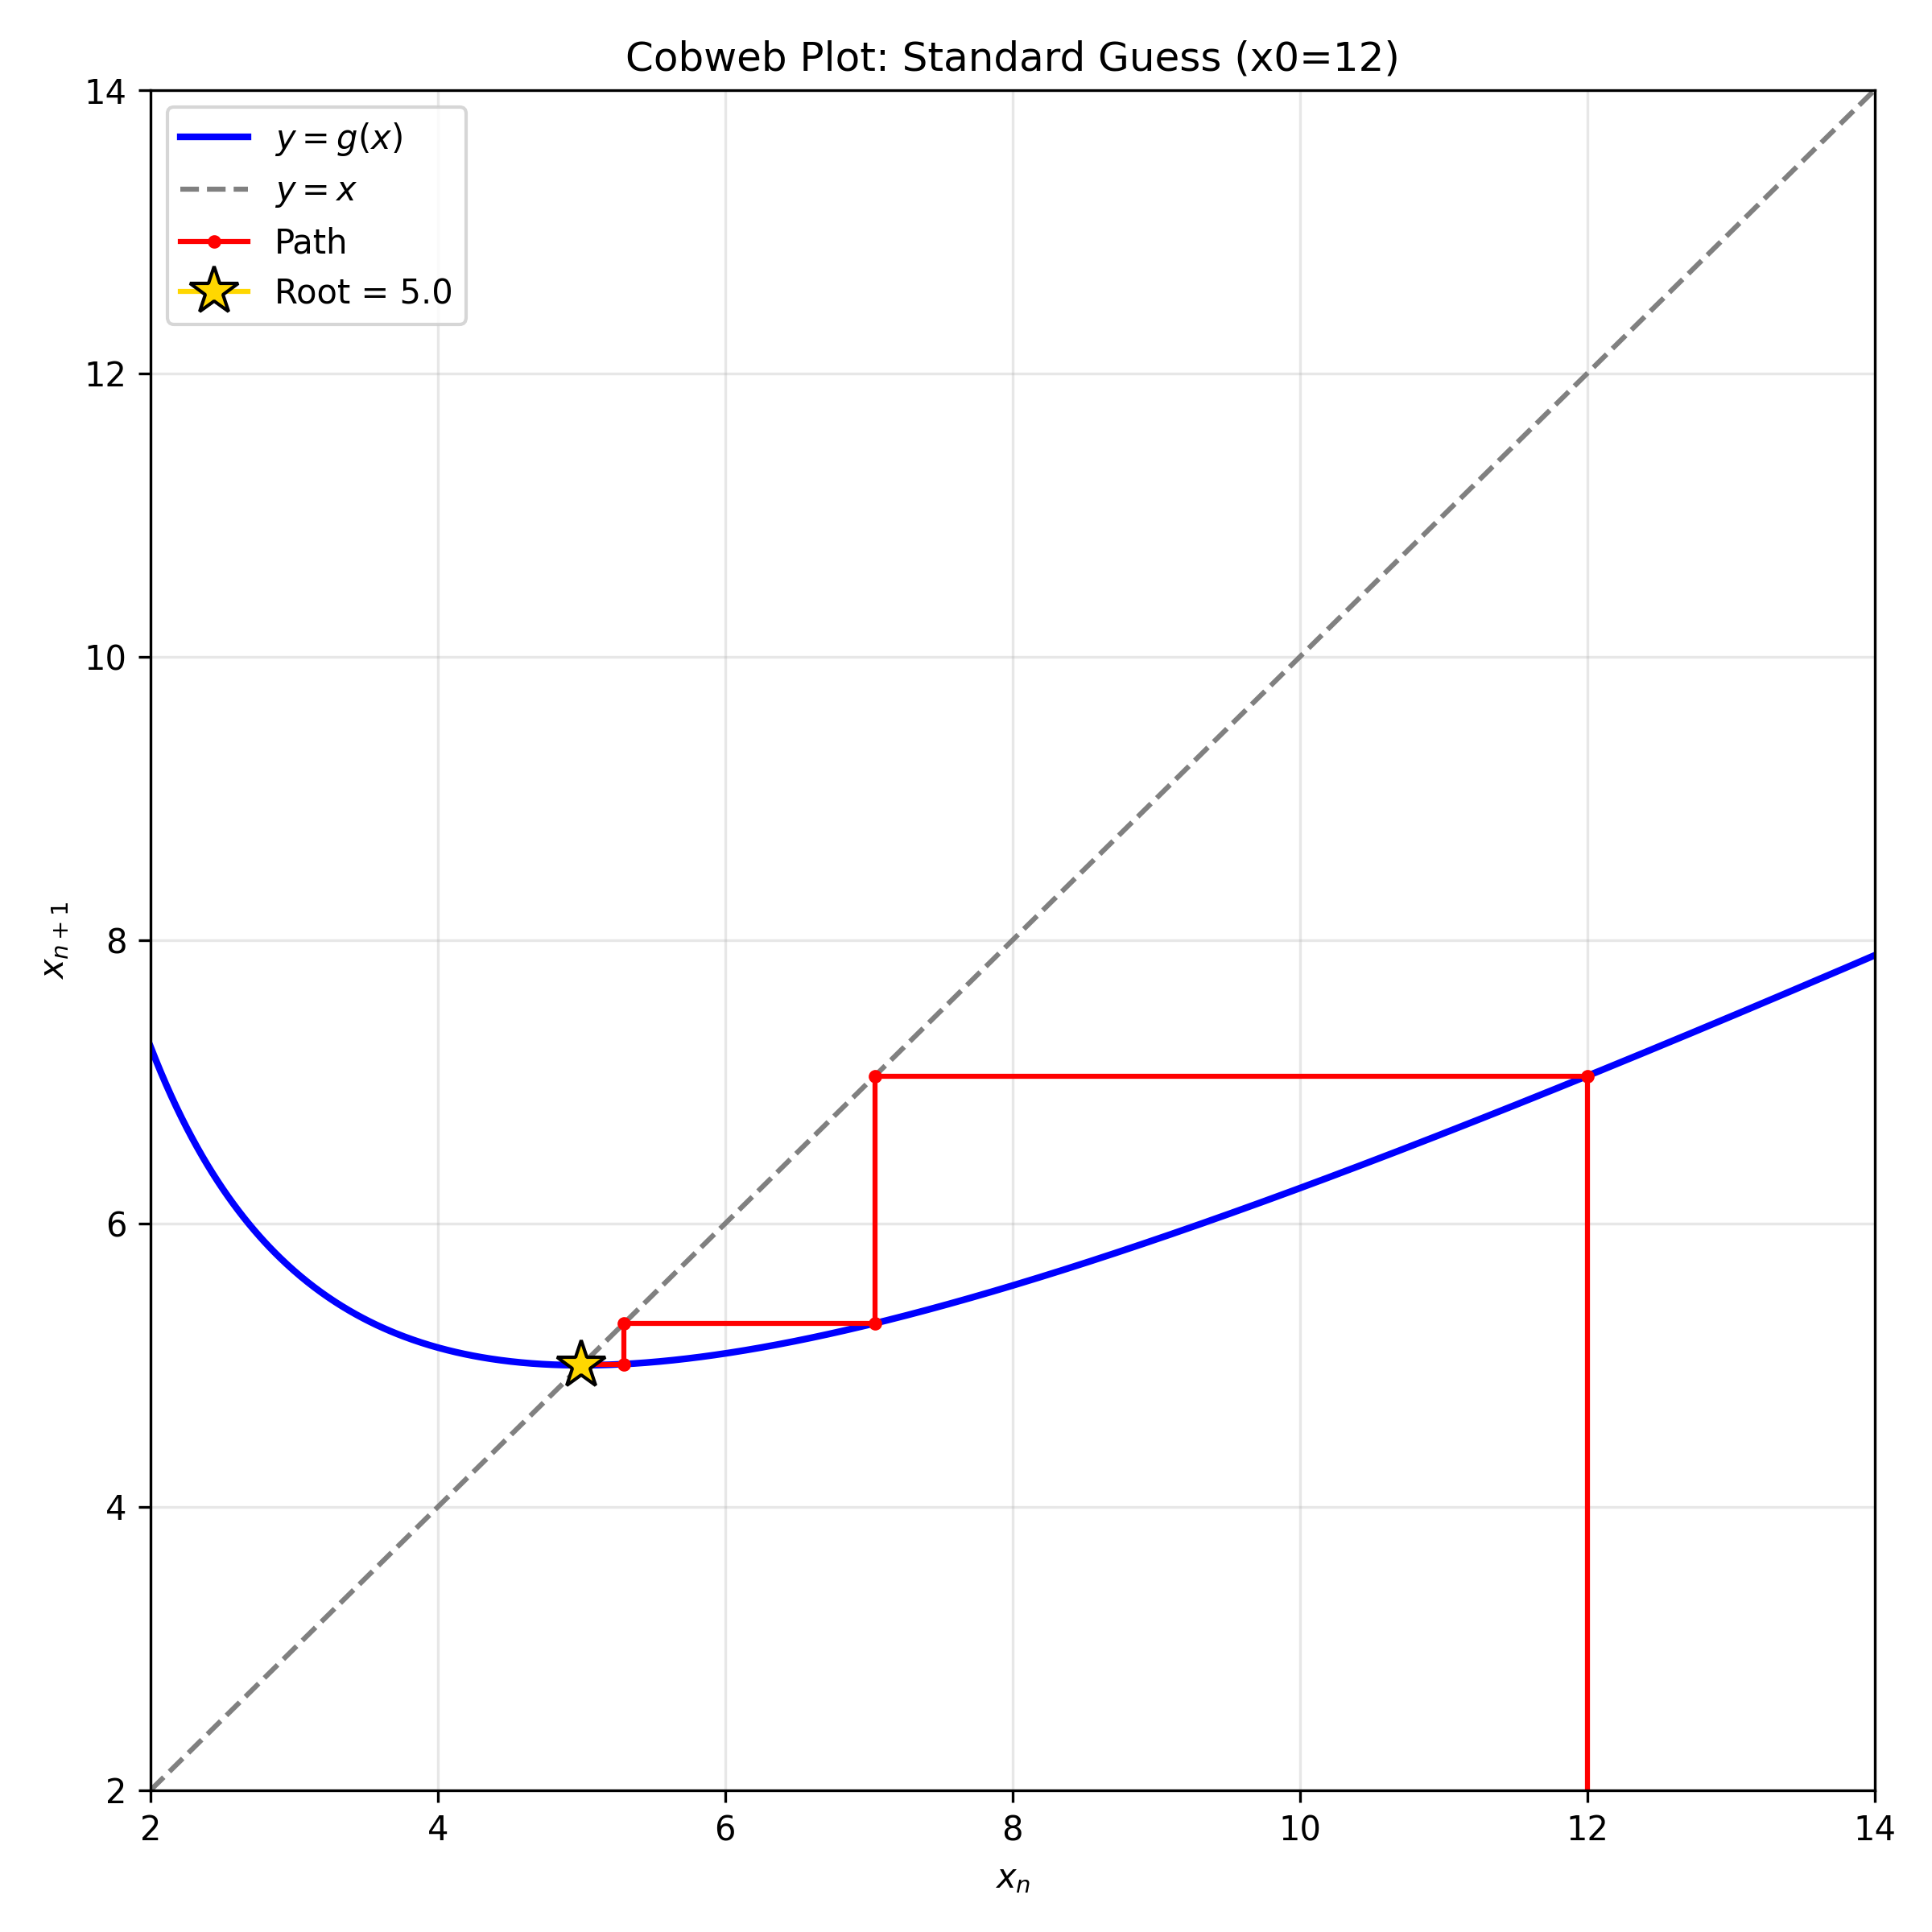
\includegraphics[height=0.7\textheight]{../figs/plot4_cobweb_std.png}
    \end{center}
\end{frame}

% Method 3: Cobweb Plot (Close to zero)
\begin{frame}{Method 3: Cobweb Plot (Small Guess)}
    Starting with a guess very close to zero ($x_0 = 0.5$) causes a massive initial jump due to the $\frac{R}{x_n}$ term dominating. However, once the sequence lands to the right of the root, it quickly converges back to $x = 5$.
    \begin{center}
        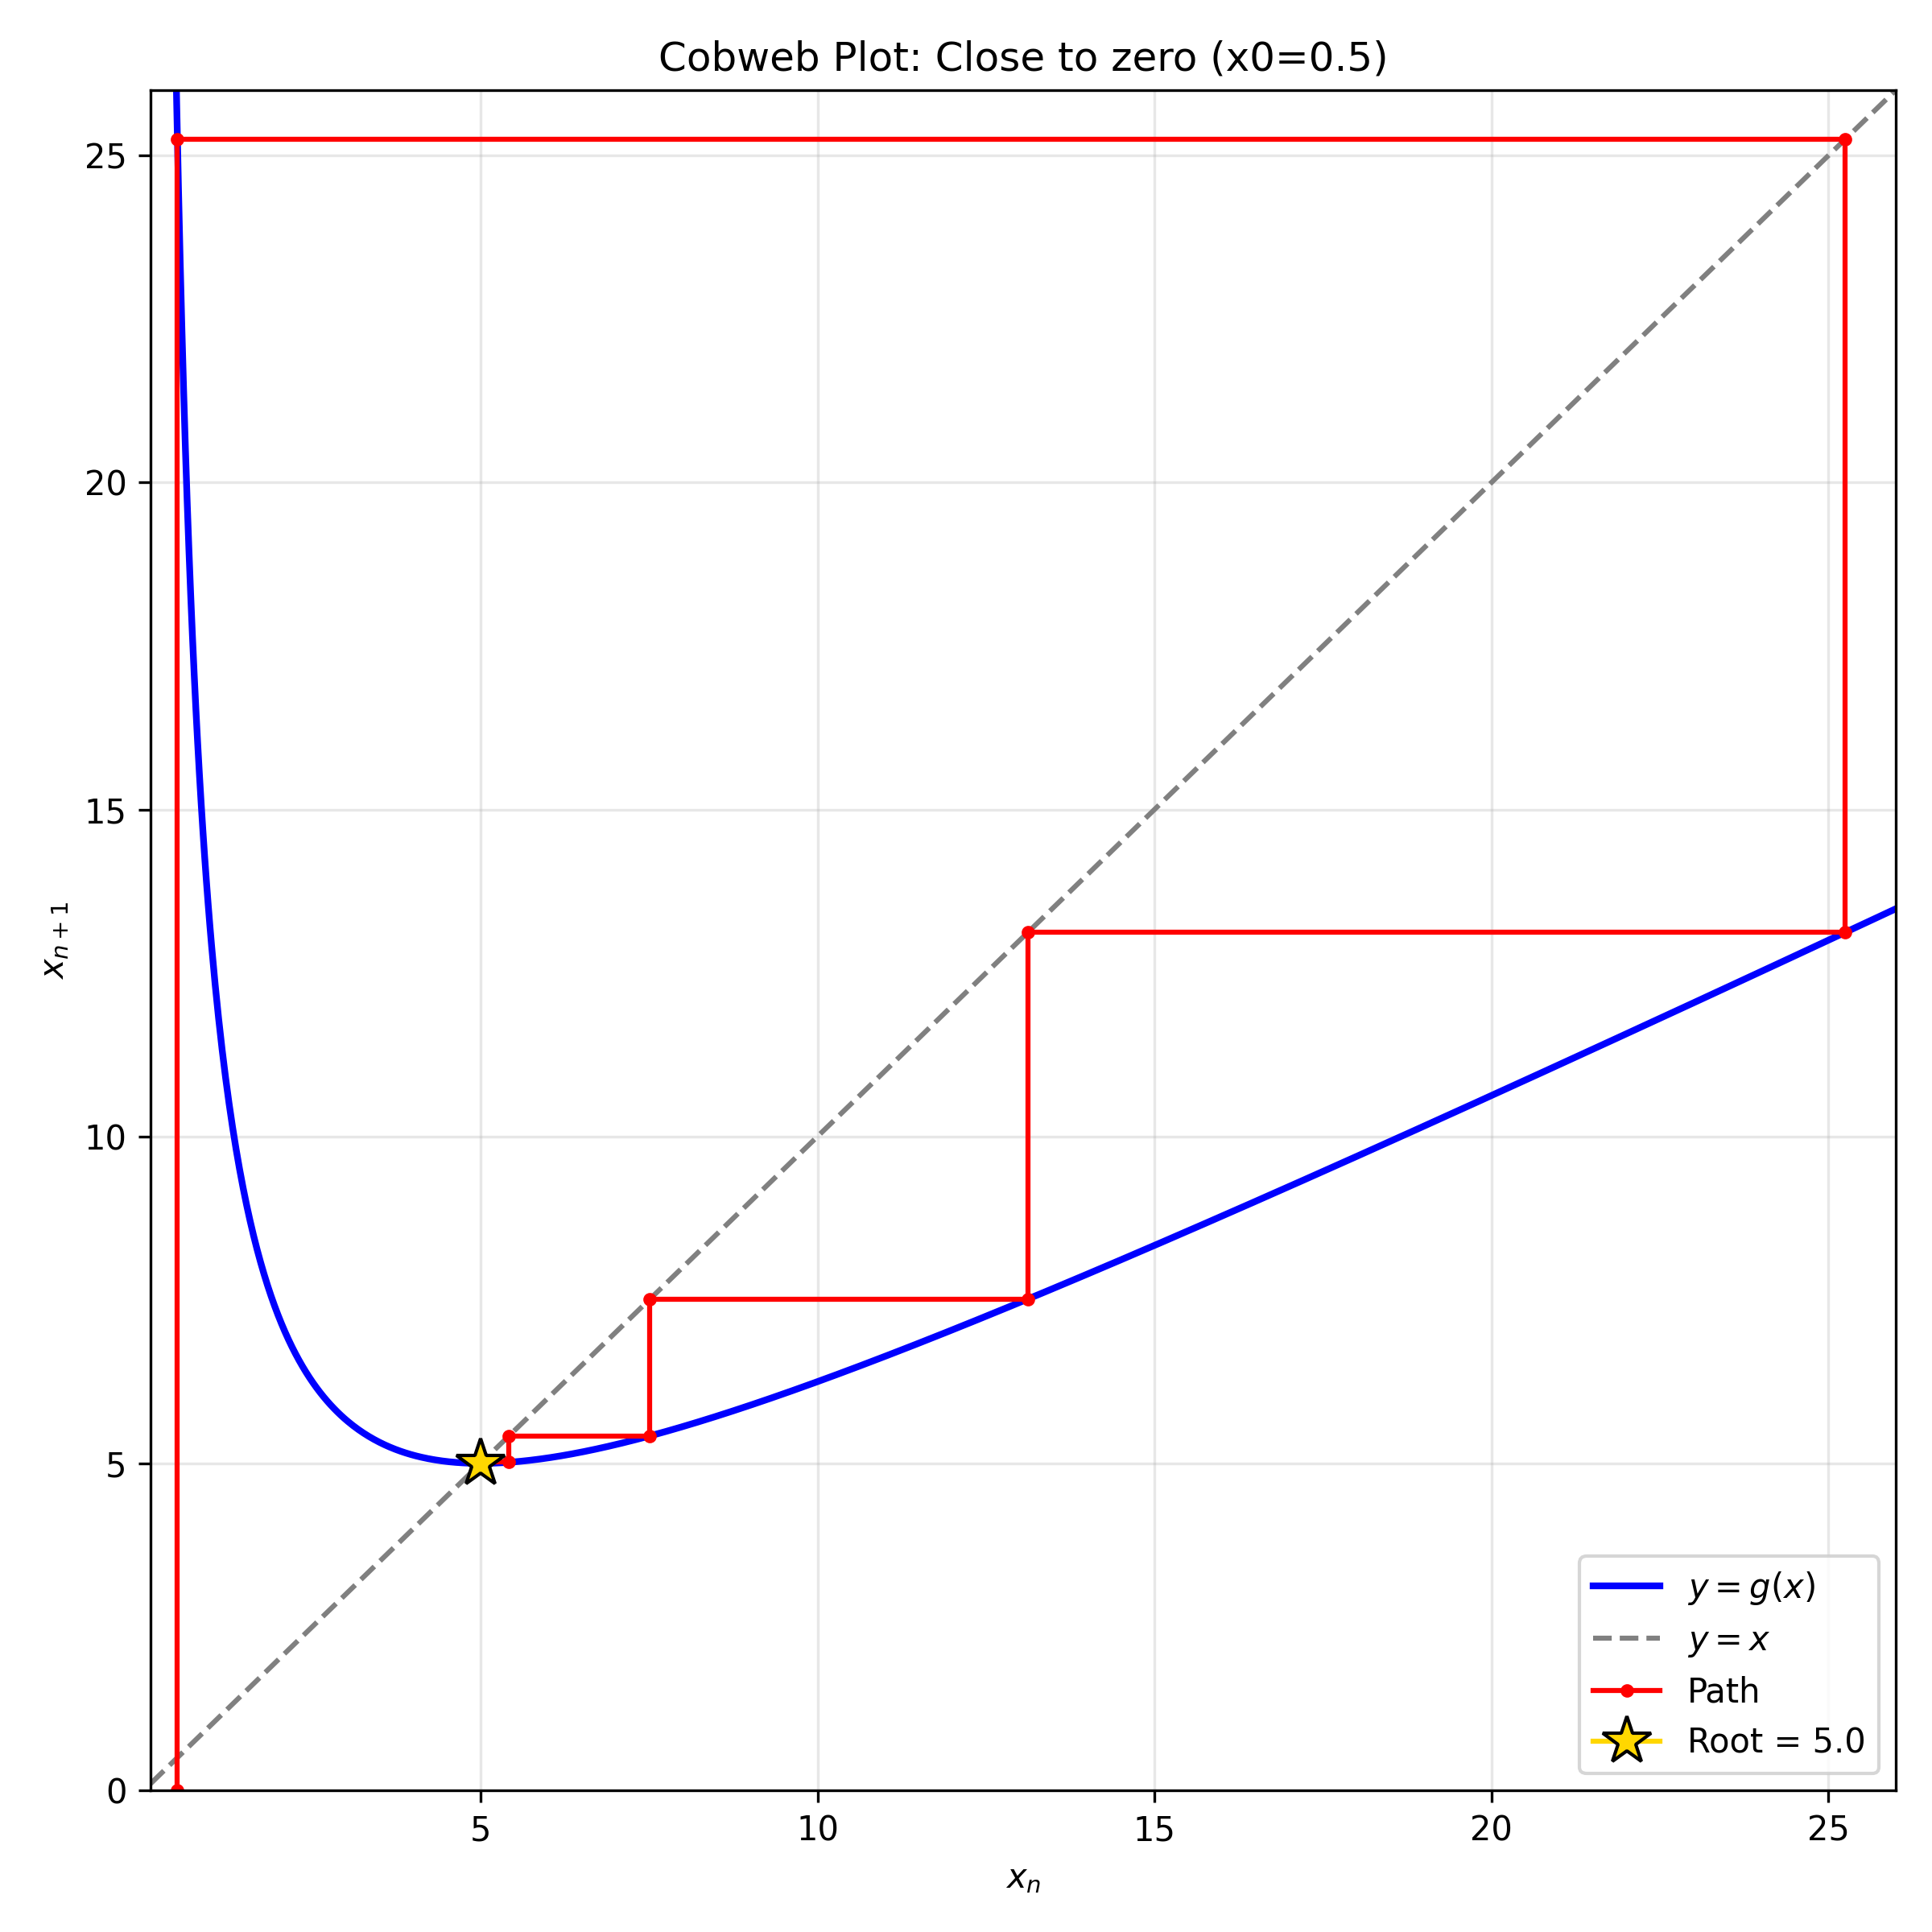
\includegraphics[height=0.7\textheight]{../figs/plot5_cobweb_small.png}
    \end{center}
\end{frame}

% Method 3: Cobweb Plot (Negative)
\begin{frame}{Method 3: Cobweb Plot (Negative Guess)}
    Because the function $g(x) = \frac{1}{2}(x + \frac{R}{x})$ is an odd function, initializing with a negative value ($x_0 = -12$) simply mirrors the process in the third quadrant, converging safely to the alternate valid root $-\sqrt{R} = -5$.
    \begin{center}
        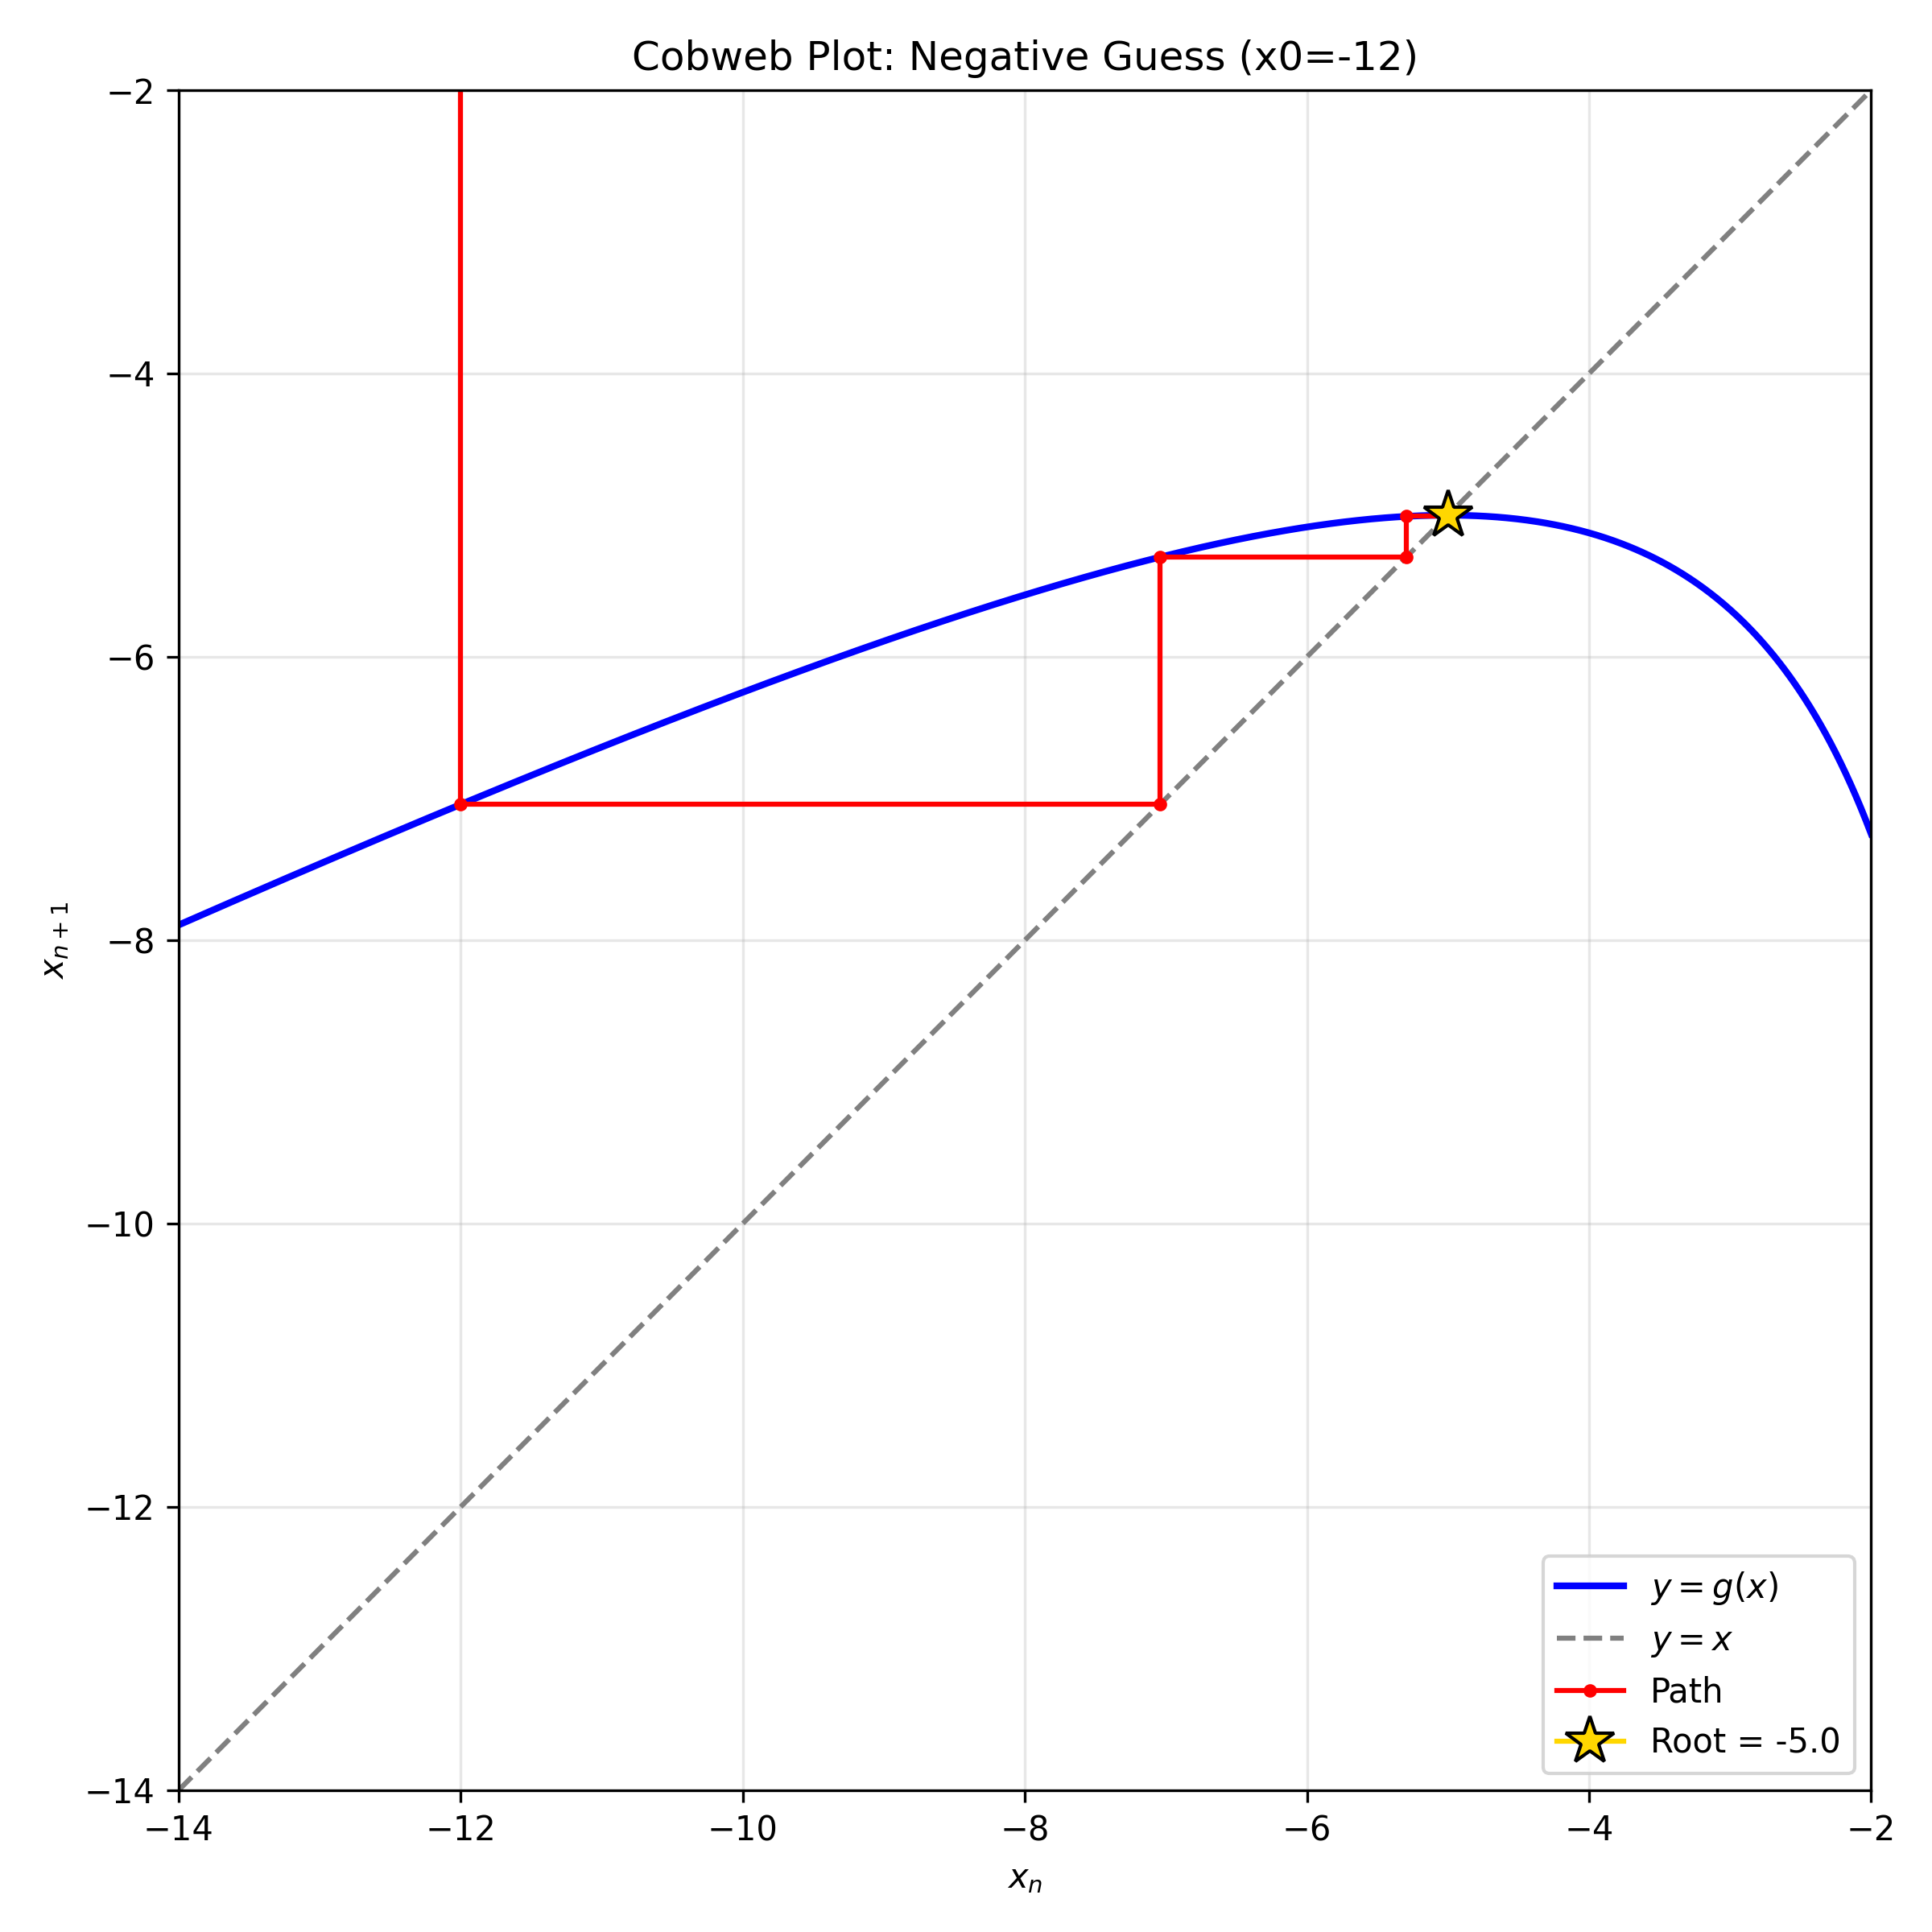
\includegraphics[height=0.7\textheight]{../figs/plot6_cobweb_neg.png}
    \end{center}
\end{frame}

% Method 3: Stability Analysis
\begin{frame}{Stability \& Convergence Bound Analysis}
    This plot visualizes the derivative $g'(x) = \frac{1}{2}(1 - \frac{R}{x^2})$. The green shaded region marks the stability bounds where $|g'(x)| < 1$. At exactly $x = \pm 5$, $g'(x) = 0$, visually confirming the superlinear (quadratic) convergence at the roots.
    \begin{center}
        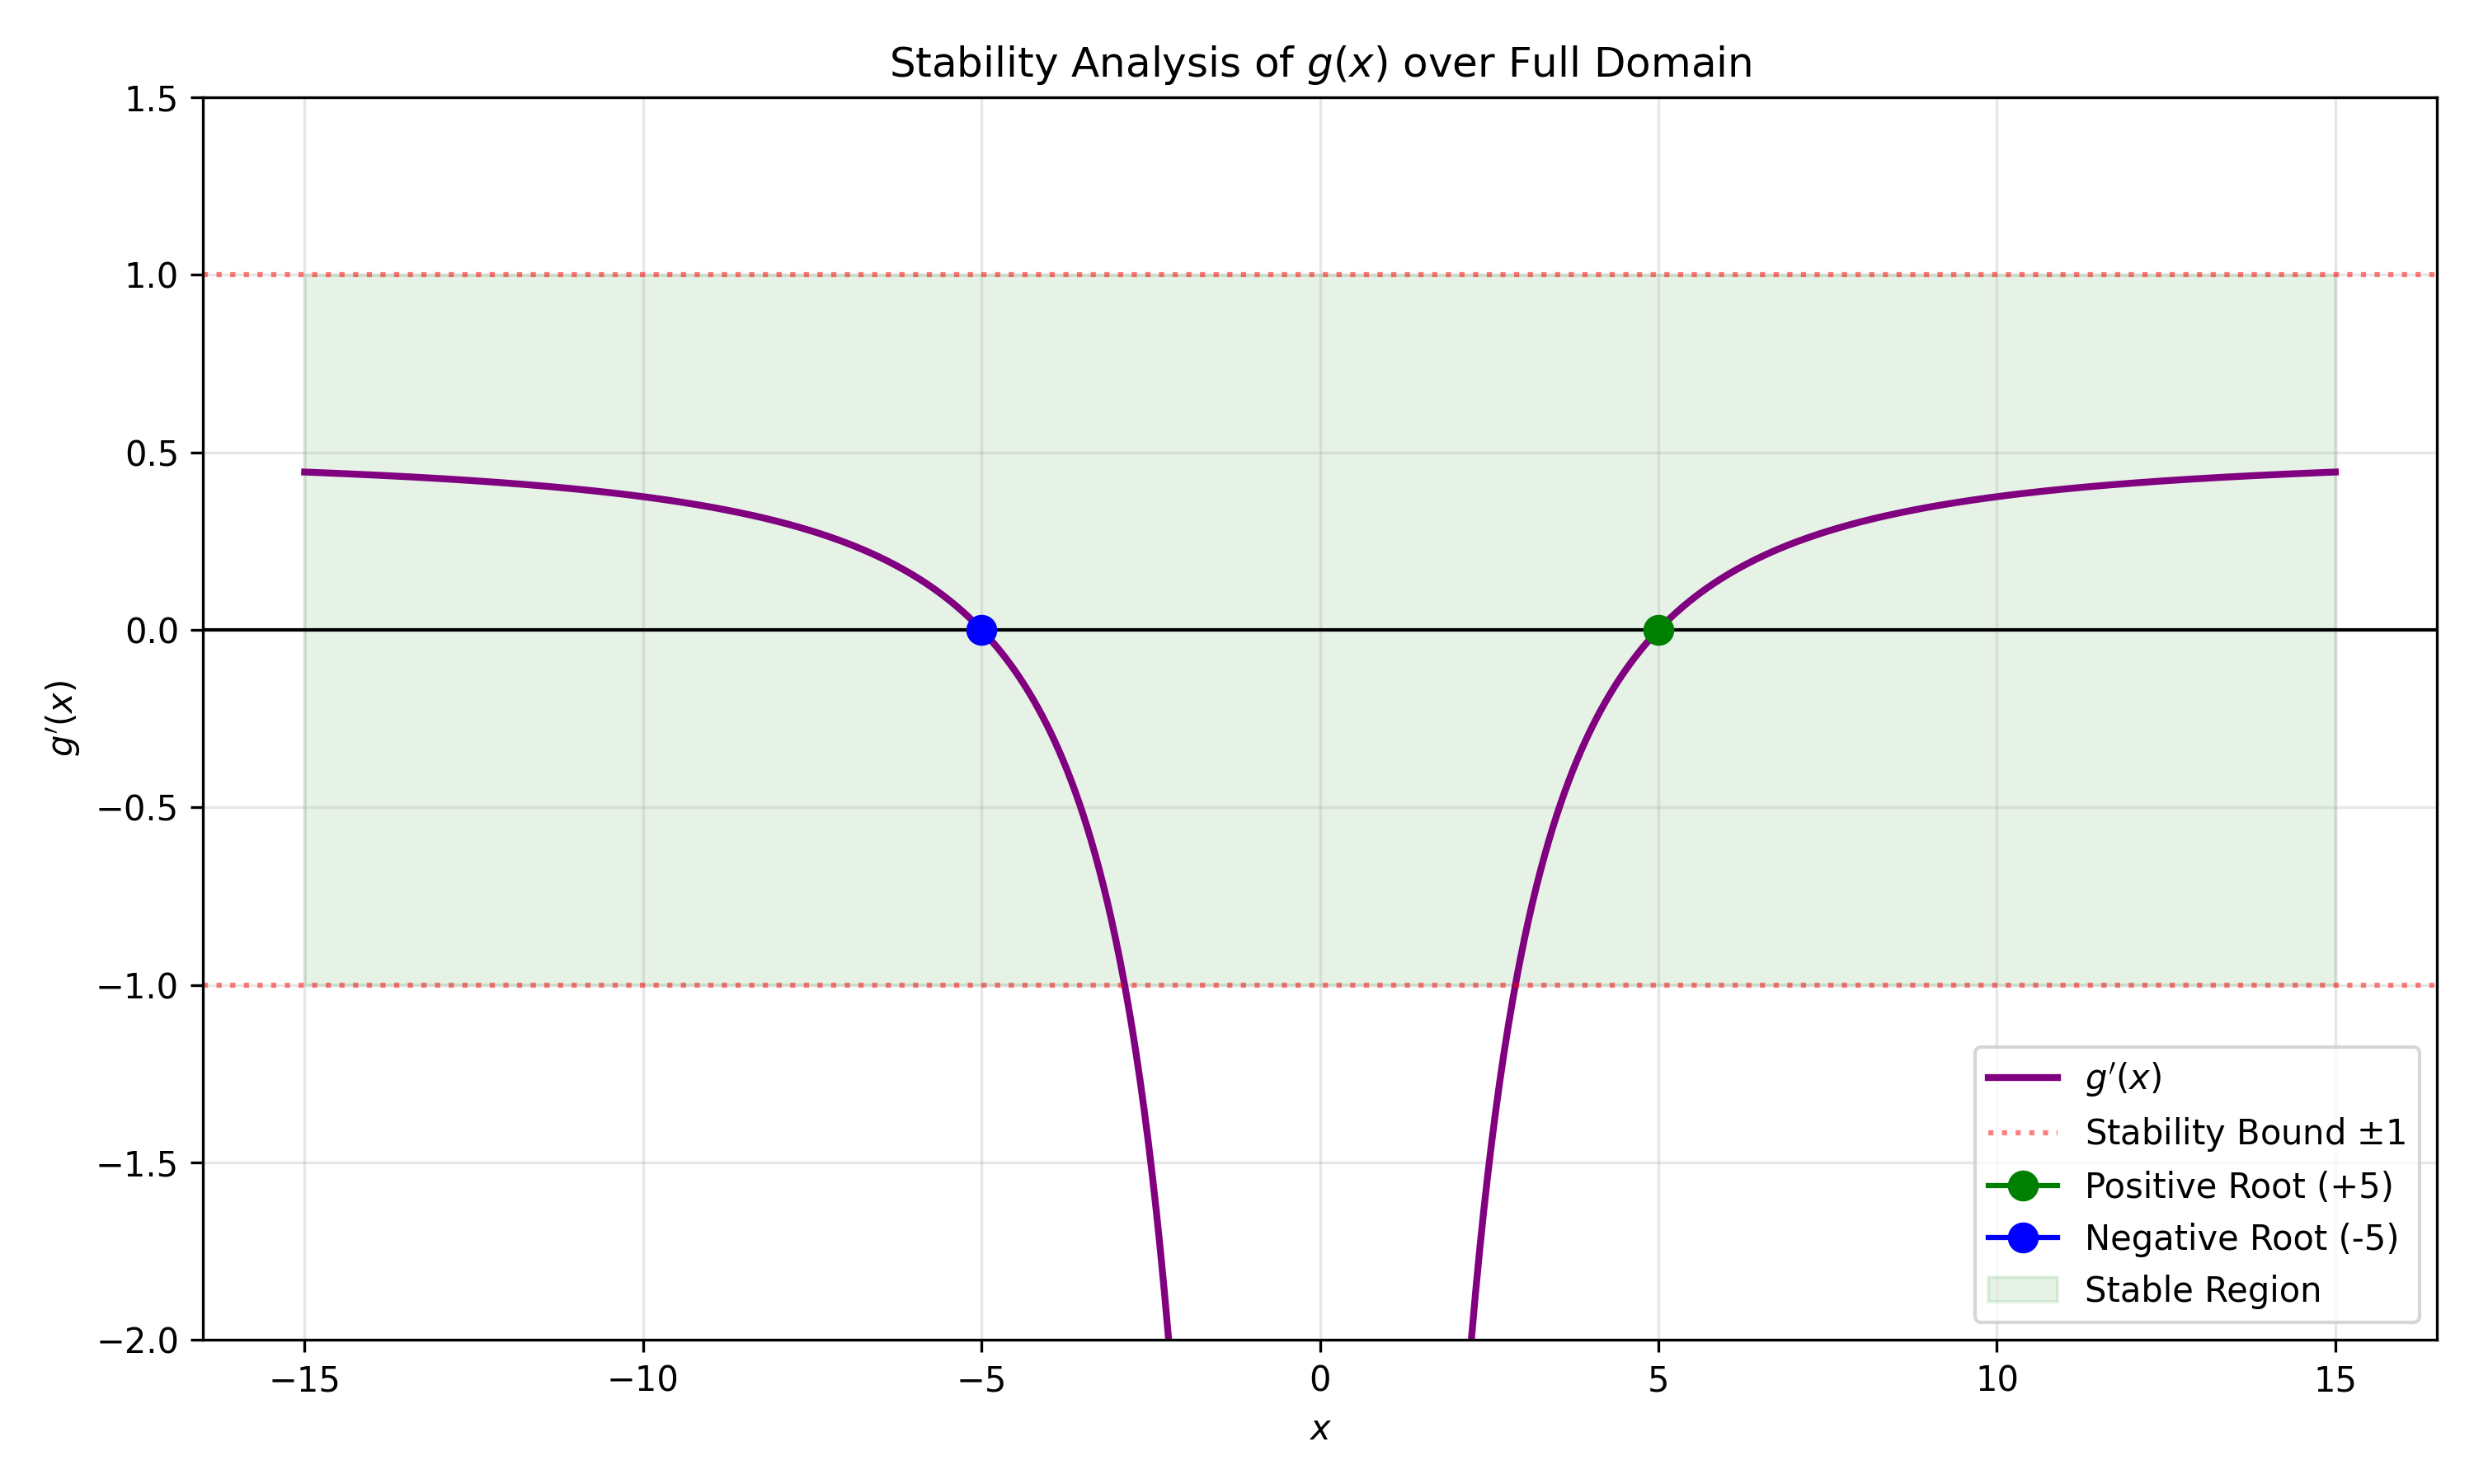
\includegraphics[width=0.85\textwidth]{../figs/plot7_stability.png}
    \end{center}
\end{frame}
\end{document}
